\chapter{Antecedentes}
\section{Estado del arte}
\subsection{Caracter�sticas de la memoria}

Tama�o de cluster que impone fat32 \cite{fat32_1} \cite{fat32_2}

\subsection{Descripci�n de equipos}
Para poder realizar los experimentos hemos contado con dos equipos en el laboratorio. Son dos equipos con procesador AMD Phenom (tm) X6 1055T, con 7'6 GiB de RAM. En los que hemos instalado Debian 6.0.6, que viene con el kernel 2.6.32-5-amd64.

Ambos dos forman parte de una red interna de \url{gf.tel.uva.es}, teniendo cada uno de ellos los siguientes hostnames:
\begin{itemize}
\item Leonardo, con la IP: 192.168.0.50.
\item Donatello, con la IP: 192.168.0.51.
\end{itemize}

Como esta red no est� accesible desde el exterior de la escuela, para poder trabajar desde casa y tener monitorizado los experimentos, hemos recurrido a los tuneles ssh y al commando screen de Linux, que detallamo en la siguiente secci�n \ref{subsec:ComoTrabajarDesdeFueraETSiT}.

\section{Utilidades}

\subsection{Comandos y herramientas utilizadas}

  - Comprar archivos: hexdump -c .iso > .txt -> comparar con meld
  - dd: bloques default 1024bytes
  - df --block-size=kB -> 1000, k -> 1024
  - cmp -l
  - diff
  - du -k == --block-size=1k == df
  - tail
  - cat
  - screen: ctrl-a + d salir, screen -r entrar
  - iotop
  - ls -l | wc -l (contar elementos)
  - od -x 1.txt muestra en hex
[1] [2]

\subsection{�Com� trabajar desde fuera de la ETSiT?}
\label{subsec:ComoTrabajarDesdeFueraETSiT}
Se puede tardar d�as en conseguir resultados, para monitorizar el proceso es necesario conectarse a los equipos y poder recuperar la shell donde tenemos lanzado el script. Para ellos nos hemos ayudado del protocolo SSH y el comando screen.

\subsubsection{SSH}
SSH es un protocolo de shell remota segura. Gracias a ello podemos conectarnos al terminal de un ordenador y ejecutar ordenes en �l.

SSH usa una autenticaci�n con cable publico/privada. Si queremos conectarnos por ssh sin tener que escribir la contrase�a cada vez, tenemos que generar una pareja de claves y a�adir la publica a nuestro servidor:
\begin{verbatim}
ssh-keygen -t rsa -b 2048
\end{verbatim}

Esto nos genera un \verb|.pub| dentro de la carpeta \verb|.ssh| y tenemos que copiar su contenido en el archivo \verb|.ssh/authorized_keys| del servidor. Con esto la pr�xima vez que nos conectemos  no tendremos que escribir la contrase�a.

\subsubsection{Tunelando con ssh}
En la escuela tenemos una arquitectura parecida a esta \ref{fig:Esquemadered}:

\begin{figure}
	\centering
		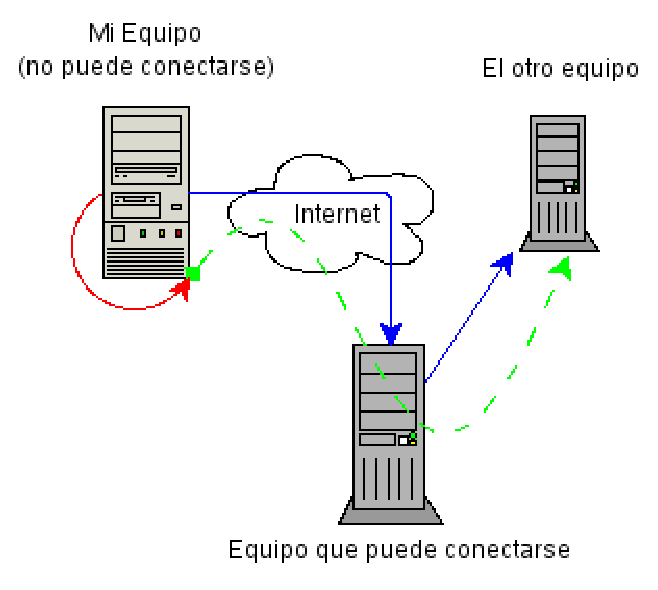
\includegraphics[width=0.60\textwidth,natwidth=299,natheight=266]{fig/tunel-ssh2}
	\caption{\emph{Esquema de red}}
        \label{fig:Esquemadered}
\end{figure}



http://dev.callepuzzle.com/uso-de-tuneles-ssh-y-screen/

[1] (man de linux)
[2] Programaci�n de Shell Scripts, Alberto Luna Fern�ndez y Pablo Sanz Mercado, 
